\section{Energetyka Jądrowa}

\begin{columnframe}{Dlaczego energetyka jądrowa może być rozwiązaniem?}
    \begin{column}{0.5\textwidth}
        \begin{figure}
            \centering
            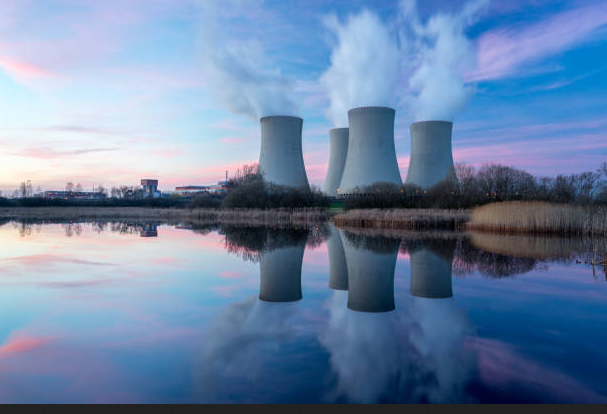
\includegraphics[width=0.6\textwidth, frame]{images/nuclear_powerplant_shutterstock.png}
        \end{figure}
    \end{column}
    \begin{column}{0.5\textwidth}
        \begin{itemize}
            \item Magazynowanie CO2 wymaga dużo energii oraz ciepła
            \item Temperatura osiągalna w reaktorach jądrowych pozwala na rozszczepienie wody (o czym więcej za chwilę)
        \end{itemize}
    \end{column}
\end{columnframe}


\begin{columnframe}{Reaktory HTR (High Temperature Reactor)}
    \begin{column}{0.5\textwidth}
        \begin{itemize}
            \item Większość reaktorów jądrowych jest chłodzona płynem (taniej, łatwiej)
            \item Aby osiągnąć wyższe temperatury reaktory HTR są chłodzone gazem
            \item Obecnie w Stanach nie ma żadnego reaktora HTR
        \end{itemize}
    \end{column}
    \begin{column}{0.5\textwidth}
        \begin{figure}
            \centering
            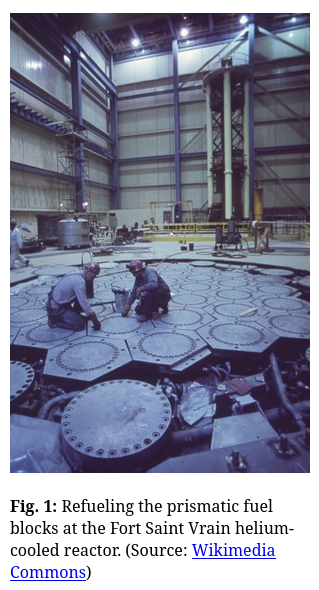
\includegraphics[width=0.6\textwidth, frame]{images/ft_st_vrain_refuel.png}
        \end{figure}
    \end{column}
\end{columnframe}


\begin{columnframe}{Reaktory HTR: UHTREX (Los Alamos, New Mexico, USA)}
    \begin{column}{0.5\textwidth}
        \begin{figure}
            \centering
            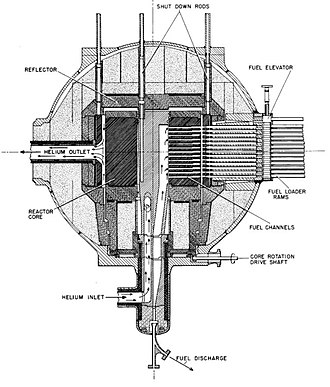
\includegraphics[width=0.6\textwidth, frame]{images/UHTREX_core_drawing.jpg}
        \end{figure}
    \end{column}
    \begin{column}{0.5\textwidth}
        \begin{itemize}
            \item Ultra-High Temperature Reactor Experiment
            \item Moc 3 MW
            \item Temperatura do 1300 \si{\degreeCelsius}
            \item Chłodzony helem
            \item 1959-1971
            \item Wymiana paliwa możliwa podczas operacji (!)
        \end{itemize}
    \end{column}
\end{columnframe}

\begin{frame}{Reaktory HTR: UHTREX (Los Alamos, New Mexico, USA)}
    \begin{figure}
        \centering
        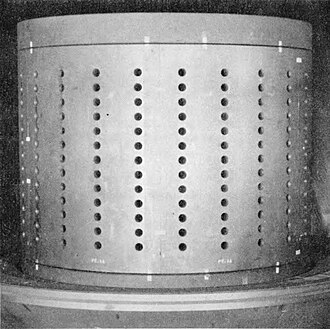
\includegraphics[width=0.6\textwidth, frame]{images/UHTREX_Moderator_graphite.jpg}
        \caption{Grafitowy moderator reaktora UHTREX}
    \end{figure}
\end{frame}



\begin{columnframe}{Reaktory HTR: Peach Bottom (USA)}
    \begin{column}{0.5\textwidth}
        \begin{figure}
            \centering
            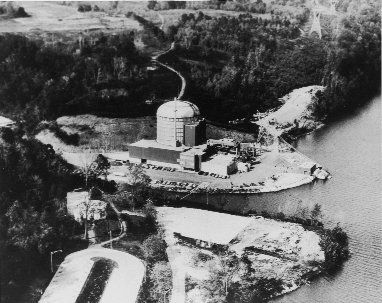
\includegraphics[width=0.6\textwidth, frame]{images/peach_bottom_aerial_view.jpg}
        \end{figure}
    \end{column}
    \begin{column}{0.5\textwidth}
        \begin{itemize}
            \item Budowa rozpoczęta w 1962 roku
            \item Typ: HTGCR
            \item wyłączony z obiegu w 1974 roku
            \item reaktor znajdował się w miejscu zagrożonym wstrząsami sejsmicznymi
            \item reaktor HTR został zastąpiony przez reaktor BWR
        \end{itemize}
    \end{column}
\end{columnframe}

\begin{columnframe}{Proponowany Reaktor VHTR (Very High Temperature Reactor)}
    \begin{column}{0.5\textwidth}
        \begin{itemize}
            \item Temperatura 750-950 \si{\degreeCelsius} (target 1000+)
            \item Helium cooled
            \item TRi-structural ISOtropic (TRISO) particles based fuel (uranium)
            \item 10 MWth to 842 MWth (termalne megawaty)
        \end{itemize}
    \end{column}
    \begin{column}{0.5\textwidth}
        \begin{figure}
            \centering
            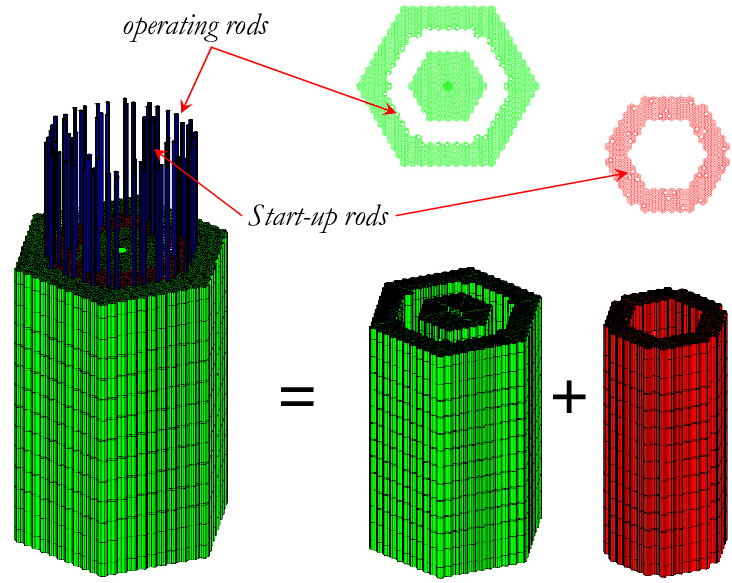
\includegraphics[width=0.6\textwidth, frame]{images/vhtr_core.png}
        \end{figure}
    \end{column}
\end{columnframe}

\begin{frame}{Proponowany Reaktor VHTR (cont.)}
    \begin{figure}
        \centering
        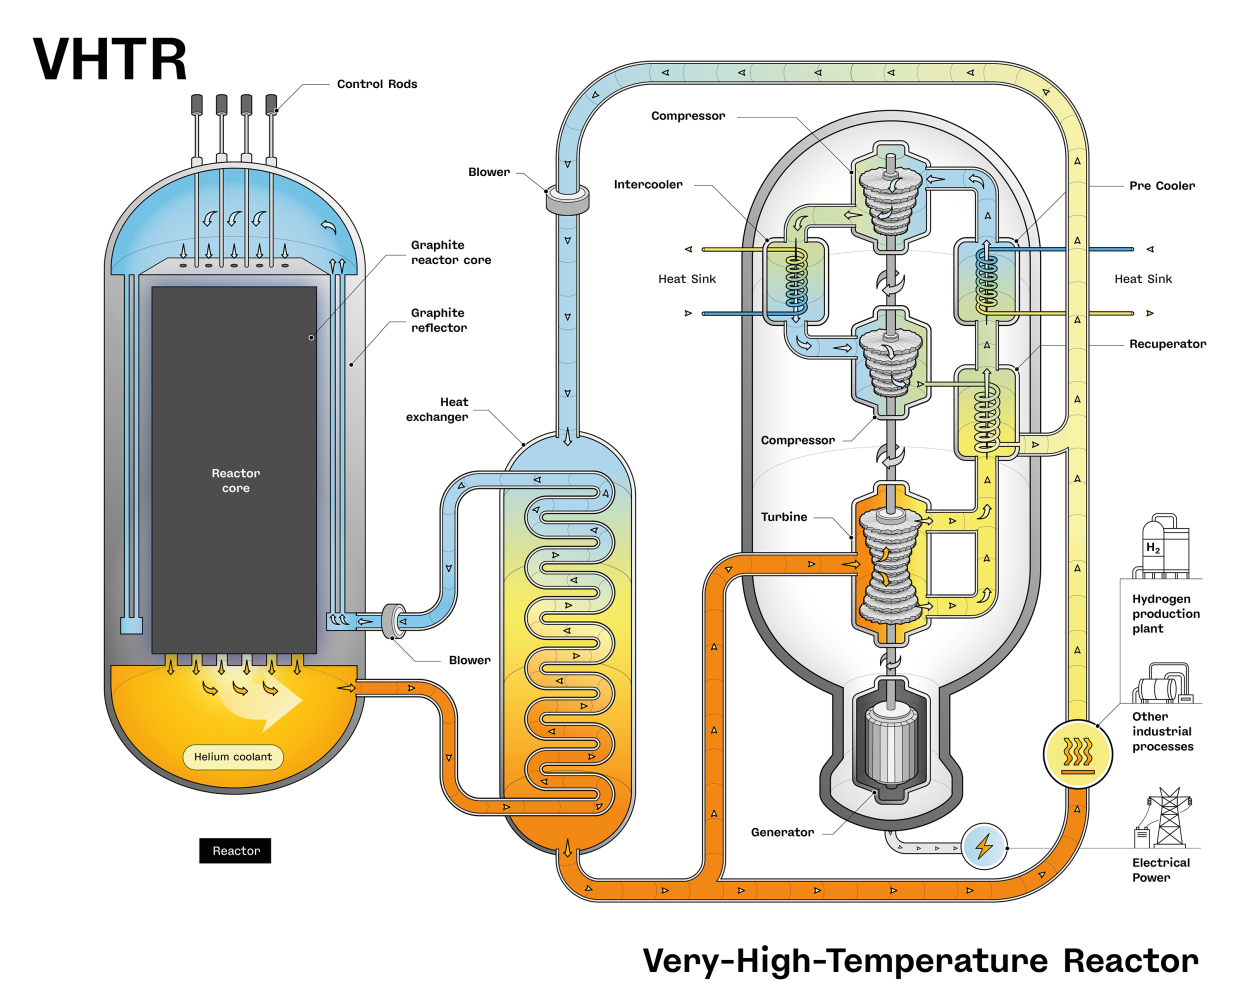
\includegraphics[width=0.7\textwidth, frame]{images/VHTR.png}
    \end{figure}
    \imagesource{https://dev.gen-4.org}
\end{frame}

\begin{frame}{Koszty produkcji energii jądrowej na tle innych źródeł}
    \begin{figure}
        \centering
        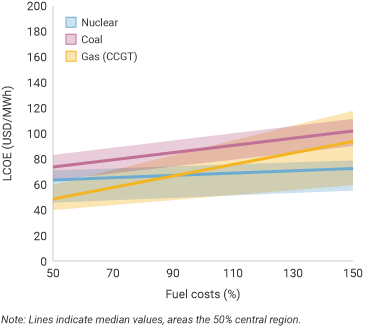
\includegraphics[width=0.6\textwidth, frame]{images/price_of_nuclear.png}
    \end{figure}
\end{frame}


\begin{columnframe}{Energetyka jądrowa w kontekście SJW}
    \begin{column}{0.6\textwidth}
        \begin{figure}
            \centering
            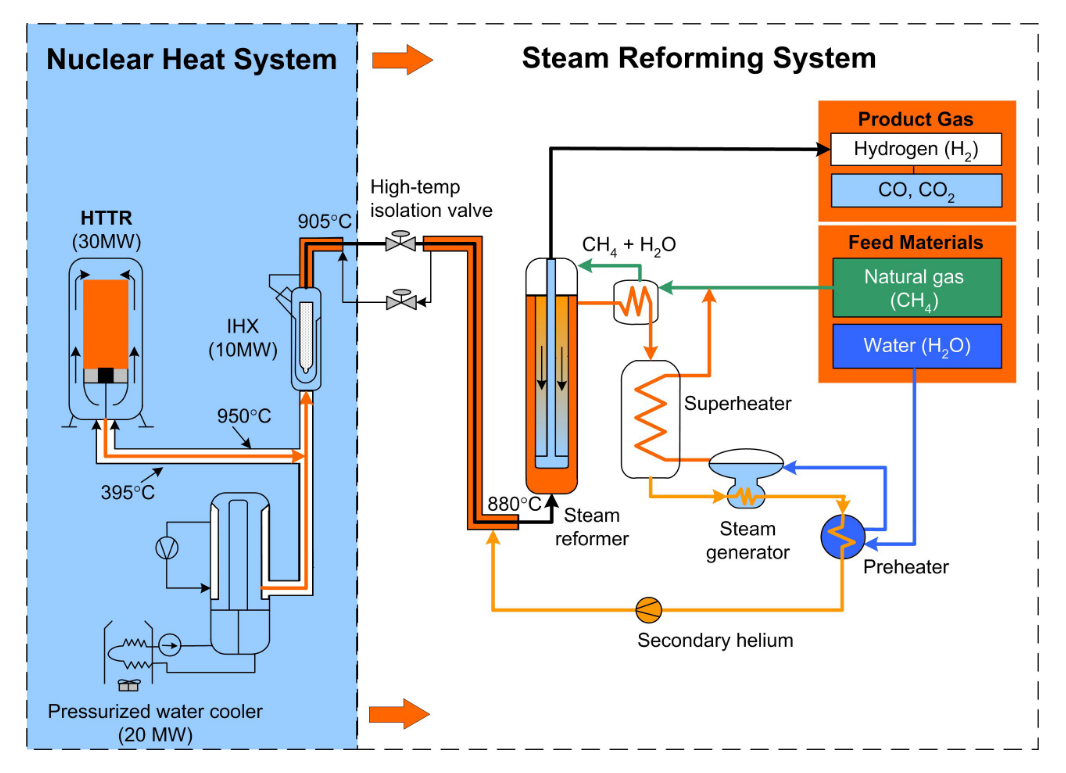
\includegraphics[width=1.0\textwidth, frame]{images/nuclear_thermolysis.png}
        \end{figure}
    \end{column}
    \begin{column}{0.4\textwidth}
        \begin{itemize}
            \item Wychwytywanie CO$_2$ wymaga dużo energii
            \item Termoliza (rozszczepienie) wody wymaga temperatury ok. 2500 \si{\degreeCelsius}
        \end{itemize}
    \end{column}
\end{columnframe}

\begin{frame}{Uran a inne źródła energii}
    \begin{figure}
        \centering
        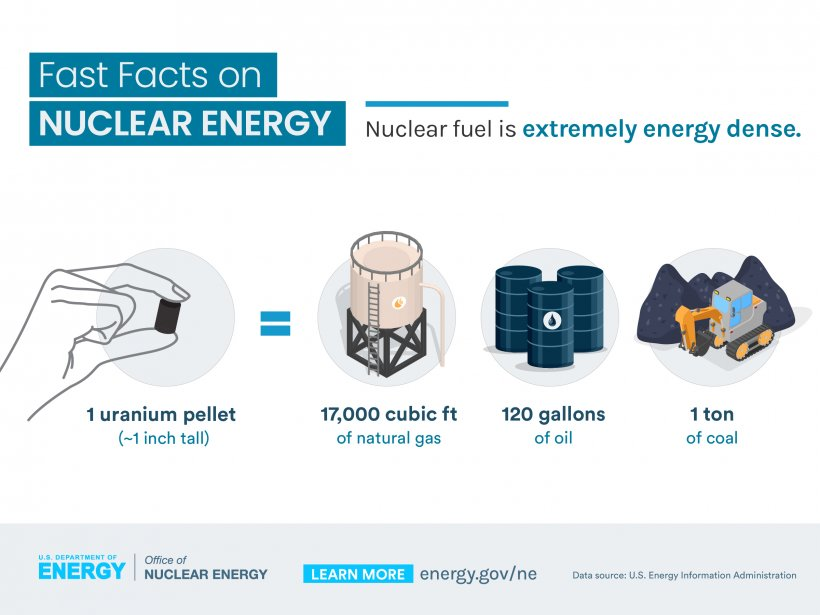
\includegraphics[width=0.7\textwidth, frame]{images/doe_uranium_propaganda.jpg}
    \end{figure}
    \imagesource{US Department of Energy}
\end{frame}

